\subsection{ASL-Skeleton3D}
\label{sec:metodologia-datasets-3d}

O ASL-Skeleton3D é um \textit{dataset} intermediário que introduz a representação em coordenadas 3D das amostras do \acrshort{asllvd}. Esse tipo de representação fornece detalhes mais precisos acerca do corpo dos indivíduos enquanto eles articulam os sinais, o que possibilita a pesquisadores em \acrshort{slr} extrair diferentes tipos de \textit{features}, explorar novas técnicas, ou ainda derivar outros novos \textit{datasets}.

Para que fosse possível projetar as amostras do \acrshort{asllvd} dentro do espaço tridimensional, adotamos uma estratégia que consiste essencialmente em combinar duas de suas perspectivas 2D perpendiculares entre si -- a vista frontal e a vista lateral -- para reconstruir uma perspectiva 3D, conforme ilustra a \autoref{fig:our-strategy-3d}. Com isso, assumimos que enquanto a vista frontal nos fornece os eixos \(x\) e \(y\), a vista lateral nos fornecerá a dimensão de profundidade, correspondente ao eixo \( z\).


% TODO: ? criar componente para sub-figuras (lembrar de formatar bordas e espaçamento horizontal, conforme padrão ABNT)
\begin{figure}[ht!]
    \centering
    \caption{\textmd{Estratégia adotada para representar as amostras no espaço 3D: as perspectivas frontal (\subref{subfig:our-strategy-3d-front}) e lateral (\subref{subfig:our-strategy-3d-side}) são posicionadas perpendicularmente para reconstruir uma perspectiva 3D (\subref{subfig:our-strategy-3d-persp}).}}
    \subcaptionbox{\label{subfig:our-strategy-3d-front}}{
        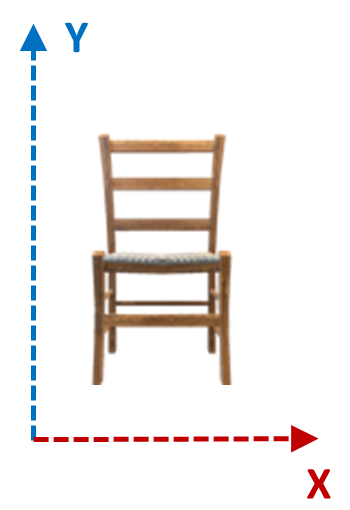
\includegraphics[height=4cm]{capitulos/metodologia/imagens/chair_front}
    }%
    % \hfill
    \subcaptionbox{\label{subfig:our-strategy-3d-side}}{
        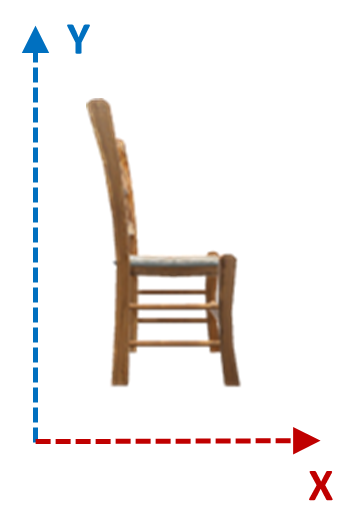
\includegraphics[height=4cm]{capitulos/metodologia/imagens/chair_side}
    }%
    % \hfill
    \subcaptionbox{\label{subfig:our-strategy-3d-persp}}{
        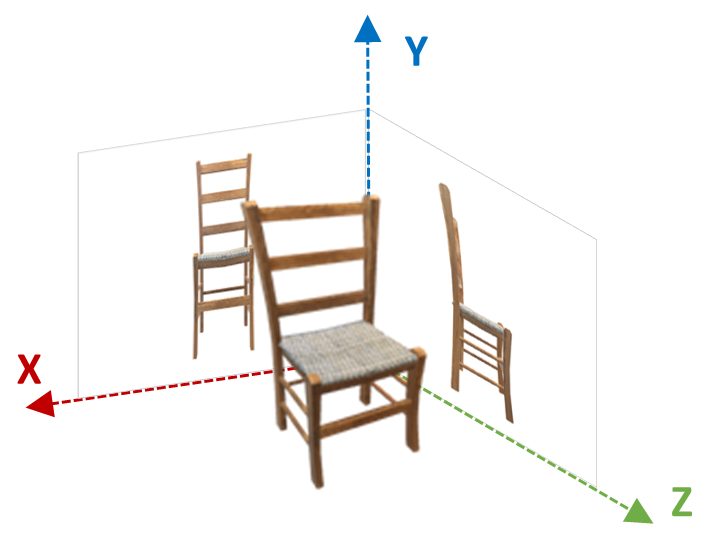
\includegraphics[height=4cm]{capitulos/metodologia/imagens/chair_perspective}
    }%
    \nomefonte{}
    \label{fig:our-strategy-3d}
\end{figure}


Uma vez definida essa estratégia, nos baseamos no processo descrito por \citeonline{amorim-2019-stgcn-sl} para realizar a estimativa dos esqueletos para os indivíduos nas amostras. Esse processo é composto pelas etapas de obtenção de amostras, segmentação dos sinais, estimativa e normalização dos esqueletos, as quais sofreram adaptações no contexto do presente trabalho para acomodar a composição de esqueletos 3D e os desafios que encontramos para isso. Discutiremos a seguir as adaptações aplicadas:

% Os passos utilizados para gerar o ASL-Skeleton3D basearam-se no processamento realizado por \citeonline{amorim-2019-stgcn-sl} na construção de um \textit{dataset} de esqueletos 2D da \acrshort{asl}. De um modo geral, eles envolvem a obtenção das amostras, a segmentação dos sinais, a estimativa e a normalização dos esqueletos. Apesar disso, várias adaptações foram necessárias a cada passo para acomodar a estratégia descrita acima e lidar com os desafios encontrados aqui, conforme discutiremos a seguir:

\begin{enumerate}
    \item \textbf{Obtenção das amostras}: nessa etapa as amostras de vídeos são recuperadas a partir dos servidores do \acrshort{asllvd}, mas no contexto atual fazemos isso para ambas as câmeras frontal e lateral.

          A saber, existem dois formatos nos quais os vídeos dessas câmeras podem ser disponibilizados: o \textit{mov}, que é compacto e mais fácil de processar; e o \textit{.vid}, que consiste no vídeo bruto, que é maior e mais pesado para baixar e processar.
          Ao analisar as amostras, identificamos que parte delas possuía ambas câmeras disponíveis nos dois formatos; para outras, cada câmera estava em um formato distinto; contudo, nos piores casos uma das câmeras estava ausente ou corrompida, fazendo com que essas amostras fossem perdidas. Lidar com essa falta de homogeneidade acrescentou uma complexidade inesperada, mas que foi contornada resultando numa perda de apenas 0,16\% das amostras originais -- ou seja, 16 amostras de um total inicial de 9.763.


    \item \textbf{Segmentação dos sinais}: compreende a segmentação das sequências de vídeos do \acrshort{asllvd} em pedaços menores, contendo um único sinal.
          Nessa etapa também reduzimos a taxa de quadros de 60 para 3 FPS, uma vez que consideramos que é pouco provável a articulação de mais de três movimentos relevantes em um único segundo.
          Isso contribuiu para reduzir em cerca de 20 vezes o número de frames a serem processados nas etapas seguintes.


    \item \textbf{Estimativa dos esqueletos 3D}: nesse momento os esqueletos dos sinalizadores são estimados utilizando-se o OpenPose para ambas as câmeras frontal e lateral. Dois esqueletos 2D são obtidos a partir disso:

          \begin{enumerate}
              \item \textit{Esqueleto frontal} (\autoref{subfig:front-side-persp-skeletons-front}), contendo as coordenadas plotadas sobre o eixos \(x\) e \(y\) que correspondem às mesmas coordenadas \(x\) e \(y\) de quando imaginamos o indivíduo representado no espaço tridimensional (vide \autoref{subfig:front-side-persp-skeletons-persp}).
                    % Essas coordenadas descrevem a mesma visão frontal que esperamos obter ao imaginar o nosso esqueleto 3D final observado de frente. Por conta disso, utilizamos essas coordenadas \(x\) e \(y\) da forma como são fornecidas para ancorar o indivíduo no espaço tridimensional. Precisaremos apenas adicionar a dimensão de profundidade.

              \item \textit{Esqueleto lateral} (\autoref{subfig:front-side-persp-skeletons-side}), que também é estimado com um par de coordenadas \(x\) e \(y\) mas que, quando posicionados perpendicularmente ao esqueleto frontal (vide \autoref{subfig:front-side-persp-skeletons-persp}), denotam a dimensão de profundidade e correspondem aos eixos \(z\) e \(y\) do indivíduo no espaço tridimensional, respectivamente. Uma vez que \(y\) já foi obtido por meio do esqueleto frontal, ele pode ser então descartado.

                    % No entanto, vamos aplicar a estratégia descrita acima e posicioná-lo perpendicularmente ao esqueleto frontal (como no ~\autoref{subfig:front-side-persp-skeletons-persp}). Nesse caso, observamos que embora o eixo \(y\) fornecido aqui contenha as mesmas coordenadas que no esqueleto frontal, o eixo \(x\) descreverá coordenadas equivalentes às de profundidade. Dessa forma, tomaremos o eixo \(x\) do esqueleto lateral como sendo o eixo \(z\) (eixo de profundidade) para o nosso esqueleto 3D final.
          \end{enumerate}

          Dessa forma, combinamos as coordenadas \(x\), \(y\) e \(z\) obtidas para dar origem ao nosso esqueleto 3D.

          \begin{figure}[ht!]
              \centering
              \caption{\textmd{Os esqueletos 2D frontal (\subref{subfig:front-side-persp-skeletons-front}) e lateral (\subref{subfig:front-side-persp-skeletons-side}) são posicionados perpendicularmente (\subref{subfig:front-side-persp-skeletons-persp}) e combinados para compor o esqueleto 3D final utilizado aqui.}}
              \subcaptionbox{\label{subfig:front-side-persp-skeletons-front}}{
                  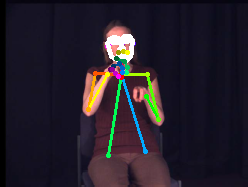
\includegraphics[height=3cm]{capitulos/metodologia/imagens/asllvd_example_front_skeleton}
              }%
              %   \hfill
              \subcaptionbox{\label{subfig:front-side-persp-skeletons-side}}{
                  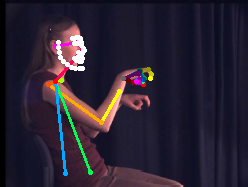
\includegraphics[height=3cm]{capitulos/metodologia/imagens/asllvd_example_side_skeleton}
              }%
              %   \hfill
              \subcaptionbox{\label{subfig:front-side-persp-skeletons-persp}}{
                  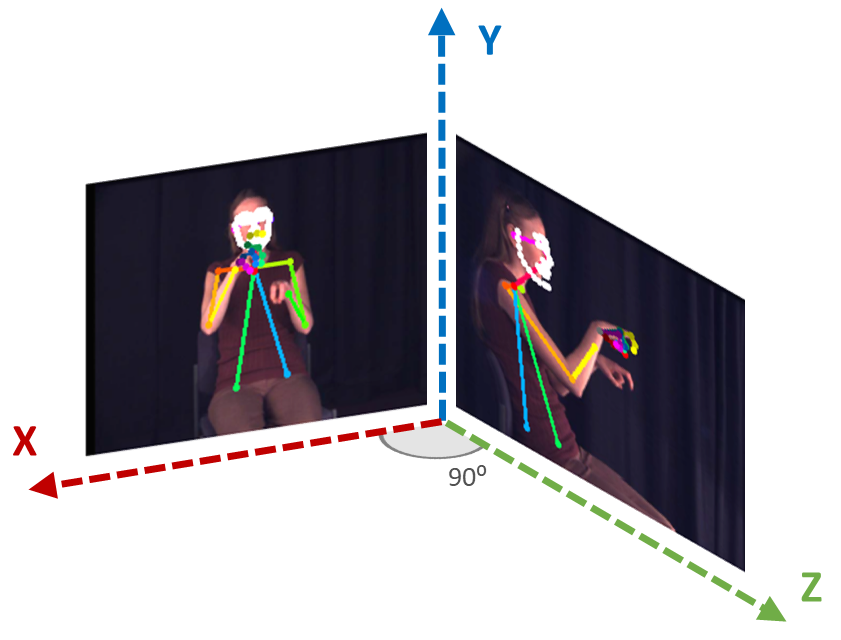
\includegraphics[height=4.5cm]{capitulos/metodologia/imagens/asllvd_front_side_perspective_skeleton}
              }%
              \nomefonte{}
              \label{fig:front-side-persp-skeletons}
          \end{figure}


    \item \textbf{Normalização dos esqueletos 3D}: por fim, os esqueletos 3D são normalizados para remover variações decorrentes do posicionamento das câmeras e dos corpos dos indivíduos. Isso é importante porque o \acrshort{asllvd} foi capturado através de diferentes seções e envolveu diferentes sinalizadores.

          Adotamos como referência para essa normalização a largura entre os ombros dos sinalizadores (vide \autoref{fig:shoulders-width}), a qual foi inspirada pela medida antropométrica de \textit{diâmetro biacromial} apresentada por \citeonline{stoudt-1970-skinfolds}. Dessa forma, a largura entre os ombros \(W_{shoulders}\) é definida aqui como a distância euclidiana \(d\) entre as coordenadas do ombro esquerdo \(S_{l}\) e do ombro direito \(S_ {r}\), conforme \autoref{eqn:shoulders-width}:

          \figura
          {fig:shoulders-width} % Label
          {capitulos/metodologia/imagens/shoulders_width} % Path
          {height=3cm} % Size
          {A largura entre ombros foi utilizada para normalizar as coordenadas nos esqueletos 3D.} % Caption
          {} % Citation

          \begin{equation}
              \label{eqn:shoulders-width}
              W_{shoulders} = d\left(S_{l}, S_{r}\right)
          \end{equation}

          Utilizando-se \(W_{shoulders}\) é possível transformar as coordenadas \(K\) do esqueleto 3D em coordenadas normalizadas \(K_{norm}\), conforme \autoref{eqn:normalized-keypoint}:

          % Normalização de pontos-chave:
          \begin{equation}
              \label{eqn:normalized-keypoint}
              K_{norm} = \frac{K}{W_{shoulders}}
          \end{equation}

\end{enumerate}


A \autoref{fig:sample-json-datasetTD} exemplifica uma amostra do ASL-Skeleton3D resultante do processamento acima, bem como suas propriedades. Observa-se no início do arquivo informações básicas extraídas do \acrshort{asllvd}, como rótulo, nome do indivíduo, sessão, cena, frames de início e fim, entre outras. Na propriedade ``frames'' estão listados os frames para aquela sequência e o esqueleto 3D estimado para cada um deles. Cada esqueleto contém grupos referentes ao ``\textit{body}'' (corpo), ``\textit{face}'' (face), ``\textit{hand left}'' (mão direita) e ``\textit{hand right}'' (mão esquerda) que, por sua vez, contêm propriedades que listam o nome da coordenada, o ``\textit{score}'' (ou acurácia) de sua estimativa e os respectivos eixos \(x\), \(y\) e \(z\).
Por exemplo, se observarmos o primeiro índice das propriedades do grupo ``\textit{body}'' veremos que ele corresponde à coordenada ``\textit{nose}'' (nariz), apresenta um \textit{score} de aproximadamente 90\% e coordenadas \(x\), \(y\) e \(z\) localizadas em 4,488, 1,696 e 2,872.

\figura
{fig:sample-json-datasetTD} % Label
{capitulos/metodologia/imagens/code_3d} % Path
{width=0.7\linewidth} % Size
{Exemplo de amostra do ASL-Skeleton3D.} % Caption
{} % Citation

O \textit{dataset} final e o código-fonte utilizado para o processamento apresentado nesta seção estão disponíveis publicamente na URL listada abaixo\footnote{Disponível em \url{http://www.cin.ufpe.br/~cca5/asl-skeleton3d}}.
